\chapter{Results}
\label{chap:results}
\section{Line Feature Projection Inacurracy}
\label{sec:linefeature_inaccuracy}
The scanned faces contain large holes in the regions of the eyes and the ears. Due to this circumstance the vertices with the most similar directions to that of the sample point may be farther away from the desired project location along the visual line from the focal point of the camera model. 
Consequently, the projected sample points of the line features may distorted along the visual line if the holes are very large and protrude in to the areas where the line features are defined, see fig. \ref{fig:linefeature_comparison}. 
\begin{figure}[h!]
    \centering
    \includegraphics[width=\textwidth]{./resources/img/linefeatures_eyes.pdf}
    \caption{Line Features}
    \label{fig:linefeature_comparison}
\end{figure}
On the different scans the quality of the projected line features varies significantly, because each scan has different holes. If a scan contains large holes one can say overall that the distortion of the projected line features increases with the amount of sampled points. 
An easy workaround to this problem is to reduce the amount of sampled points. By using only 5-10 sample points per curve most datasets rendered near perfect results. 
However, when the holes are too large this workaround also fails, slight distortions can be made out in fig. \ref{fig:linefeature_comparison} top right. This means that only one or two points are a bit off the desired position.
If the distortions are moderate they are accounted for by the additive Gaussian Noise in the joint distribution \ref{sec:noisemodel}.
However, as long as the method is dependent on the data from the scans - the size of the holes in the meshs - it lacks generality and generality is exactly the basis for feasible and reproducable registration results.\\

\section{The Effect of Line Features}
In this section we illustrate the effect of the line features on the registration results.
For this purpose we compare the feature regions of registered templates with and without line features with the respective target. We use close-up images of the various feature regions for a qualitative comparison. A detailed description of each figure is delivered in the captions.
\begin{figure}[h!]
    \centering
    \includegraphics[width=.9\textwidth]{./resources/img/00029_eyes_comparison.pdf}
\caption{A comparison of the fitting results concerning the eyes. The first image displays the eyes in the registered template without line features. The second image has been registered with line features. As one can see the eyes in the top image are in the right position, because the displacement of the corners is defined by the given landmarks. However, compared to the middle image the contours of the eyes are very different. The incorporation of line features in the middle
image has lead to a better deformation according to the eyes of the target mesh, displayed at the bottom.}
\label{fig:fiteyes}
% reference in text by \ref{$figure-name}
\end{figure}

\begin{figure}[h!]
    \centering
    \includegraphics[width=.8\textwidth]{./resources/img/00029_mouth_comparison.pdf}
    \label{fig:00029_mouth_comparison}
    \caption{At the top again is the mouth fitted without line features and beneath the one with line features. The lips in the top image are considerably thinner although the position of the mouth is of course correct due to the displacement of the landmarks in marked at the corners of the mouth. The lips in the middle image are fuller an match the mouth of the target better in this respect. However, the lower lip of the target appears to be bimodal while the lip of the fit with
    line features is still unimodal as in the template mesh.}
\end{figure}
\pagebreak

\begin{figure}[h!]
    \centering
    \includegraphics[width=\textwidth]{./resources/img/00029_left_ear_comparison.pdf}
\caption{Ears}
\label{fig:fitears}
\caption{A comparison of the fitting results of the ears. The image on the left hand side is the fit without line features and the image on the right hand side is the fit using line features. The target is displayed between the two. The ear on the left is narrower than the ear of the target and the ear of the fit using line features. Furthermore, the rather straight upper contour of the target is more closely matched using line features.}
% reference in text by \ref{$figure-name}
\end{figure}

\subsection{Visualized Distance}
To illustrate the overall quality of registration we show distance maps of the residual difference after registration. These are obtained by taking the differences of the nearest points in the deformed template and the target mesh.
\begin{figure}[h!]
    \centering
    \includegraphics[width=.8\textwidth]{./resources/img/00029_distmap.pdf}
    \label{fig:00029distmap}
    \caption{Distance face of fit displayed in fig. \ref{fig:00029fit} with a range of 0-3 millimeters (mm) from blue to red. As can be seen that after registration most large residuals remain for the holes in the target mesh. The chin region is the only facial regions that has not been matched very accurately. In the area of the line features the distances are very small.}
% reference in text by \ref{$figure-name}
\end{figure}
\begin{figure}[h!]
    \centering
    \subfloat[Target mesh with projected template texture]{\includegraphics[width=\textwidth]{./resources/img/00303_textured_target.pdf}}\\
    \subfloat[Deformed template fitted to the target]{\includegraphics[width=\textwidth]{./resources/img/00303_fit.pdf}}\\
    \subfloat[Distance map]{\includegraphics[width=\textwidth]{./resources/img/00303_distmap.pdf}}
    \caption{This figure shows the fit of the template mesh to a different target face and the distance map in a range of 0-3 millimeters from blue to red.}
\label{fig:00303fit}
% reference in text by \ref{$figure-name}
\end{figure}

\begin{figure}[h!]
    \centering
    \subfloat[Distance image of the mouth of fit shown in \ref{fig:00029fit}]{\includegraphics[width=.4\textwidth]{./resources/img/00029_dist_mouth_0_1_cropped.pdf}}\quad
    \subfloat[Distance image of the mouth of fit shown in \ref{fig:00303fit}]{\includegraphics[width=.4\textwidth]{./resources/img/00303_dist_mouth_0_1_cropped.pdf}}
    \label{fig:distmaplips}
    \caption{These distance images depict the mouth region of two different fits of the deformed template to the two targets that have been used as examples. Both distance images are on a scale of 0-1mm [blue, red]. The fit of the lips is better in a) where the area along the contour lines of the lips is mostly light blue. In b), however, the distances in the region of the lips often exceeds 1mm and quality of the fit is not as good.}
\end{figure}

\begin{figure}[h!]
    \centering
    \subfloat[Distance image of the eyes of fit shown in \ref{fig:00029fit}]{\includegraphics[width=.8\textwidth]{./resources/img/00029_dist_eyes_0_1_cropped.pdf}}\\
    \subfloat[Distance image of the eyes of fit shown in \ref{fig:00303fit}]{\includegraphics[width=.8\textwidth]{./resources/img/00303_dist_eyes_0_1_cropped.pdf}}
    \label{fig:distmapeyes}
    \caption{Again both distance images are shown on a scale of 0-1mm [blue, red]. The fit in a) has a lot of red areas, because the target mesh has large holes in the region of the eyes and along both sides of the nose and on top of the nose. The bottom inner contour of the left eye is however matched very well. The same can be said for b). Here, the bottom inner contour of the right eye is also matched accurately.}
\end{figure}

\subsection{Caricatures}
In this section we present caricatures which are obtained by increasing the deformation of the template for a specific registration result. By adding the deformation field multiplied by a scaling parameter exceeding one to the template, the characteristics of a fit should be become more prominent without causing too much unnatural distortions. 
\begin{figure}[h!]
    \centering
    %\subfloat[fit]{
\includegraphics[width=\textwidth]{./resources/img/00029_fit.pdf}}\\
    \subfloat[scaling factor 1.3]{\includegraphics[width=.9\textwidth]{./resources/img/00029_caricature_1_3.pdf}}\\
    \subfloat[scaling factor 1.6]{\includegraphics[width=.9\textwidth]{./resources/img/00029_caricature_1_6.pdf}}\\
    \subfloat[scaling factor 2]{\includegraphics[width=.9\textwidth]{./resources/img/00029_caricature_2.pdf}}\\
    \caption{Caricatures of the fit in fig. \ref{fig:00029fit} with different parameter values. With an increasing scaling factor the mouth and the nose are twisted more to the left while the ears become pointier. The eyelids are shut more and more with each step. Also a fold begins developing to both sides of the head. This artifact is caused by the increase of the minimal displacements of the template mesh vertices which have no corresponding vertices on the target
mesh and are not completely ignored by the Tukey estimator.}
\label{fig:00029_caricature}
% reference in text by \ref{$figure-name}
\end{figure}
As can be made out in the shown figures artifacts supressed by the robust estimator become visible with an increase in the scaling factor.

\begin{figure}[h!]
    \centering
    \subfloat[scaling factor 1.3]{\includegraphics[width=.9\textwidth]{./resources/img/00303_caricature_1_3.pdf}}\\
    \subfloat[scaling factor 1.6]{\includegraphics[width=.9\textwidth]{./resources/img/00303_caricature_1_6.pdf}}\\
    \subfloat[scaling factor 2]{\includegraphics[width=.9\textwidth]{./resources/img/00303_caricature_2.pdf}}
    \caption{Caricatures of fit in \ref{fig:00303fit} for three different scaling factors. Here, the exageration of a slightly hooked nose can be observed. In this case the face is bent slightly to the right and lips are pressed together and foreward. The folds on both sides of the head are prominent than in the other example.} 
\label{fig:00303_caricature}
% reference in text by \ref{$figure-name}
\end{figure}

\begin{comment}
\subsection{Effects of the Covariance Function}
A Gaussian Kernel
00125 - scan of old man --> wrinkles can't be modelled through this smooth definition of covariance - adjust covariance function
\end{comment}

